\documentclass{beamer}
%
% Choose how your presentation looks.
%
% For more themes, color themes and font themes, see:
% http://deic.uab.es/~iblanes/beamer_gallery/index_by_theme.html
%


\mode<presentation>
{
  \usetheme{Madrid}      % or try Darmstadt, Madrid, Warsaw, ...
  \usecolortheme{default} % or try albatross, beaver, crane, ...
  \usefonttheme{default}  % or try serif, structurebold, ...
  \setbeamertemplate{navigation symbols}{}
  \setbeamertemplate{caption}[numbered]

} 
\usepackage{amsmath,amssymb,amsthm,graphicx,float,subfigure,cite, pdflscape,color,setspace, xspace}
\usepackage{multimedia}
\usepackage[english]{babel}
\usepackage[utf8x]{inputenc}
\usepackage{hyperref}
%\hypersetup{
%	colorlinks   = true, %Colours links instead of boxes
%	urlcolor     = blue, %Colour for external hyperlinks
%	linkcolor    = blue, %Colour of internal links
%	citecolor   = red %Colour of citations
%}
\renewcommand{\familydefault}{\sfdefault}  % say no to serif
%\usepackage{media9}

\newcommand{\ca}{Ca$^{2+}$\xspace}

\title[Modelling \ca dynamics]{Using GNU parallel: An introduction}
\author[Emma McIvor]{Emma McIvor}
\institute{University of Nottingham}
\date{\today}

\begin{document}

\begin{frame}
  \titlepage
\end{frame}

% Uncomment these lines for an automatically generated outline.
%\begin{frame}{Outline}
% \tableofcontents
%\end{frame}

%%%%%%
\begin{frame}{What is GNU parallel and why use it?}
\begin{itemize}
	\item GNU parallel is a tool that can execute jobs (e.g. a script to run a simulation) in parallel using one or more computers
	\item GNU parallel is a shell script that wraps the script we want to execute which means we are not adding extra complexity into the simulation script (more complexity $\implies$ more chance of introducing errors!)
	\item This means we can run multiple simulations simultaneously which can be useful for reducing the overall computation time required e.g. doing parameter scans
	\item To use GNU parallel the simulations must be able to be run independently
\end{itemize}
\end{frame}

\begin{frame}{Example: Creating a basic Matlab script in parallel}
This Matlab script (\texttt{test.m}) does a simple addition and multiplication which is saved to a file:
\begin{figure}
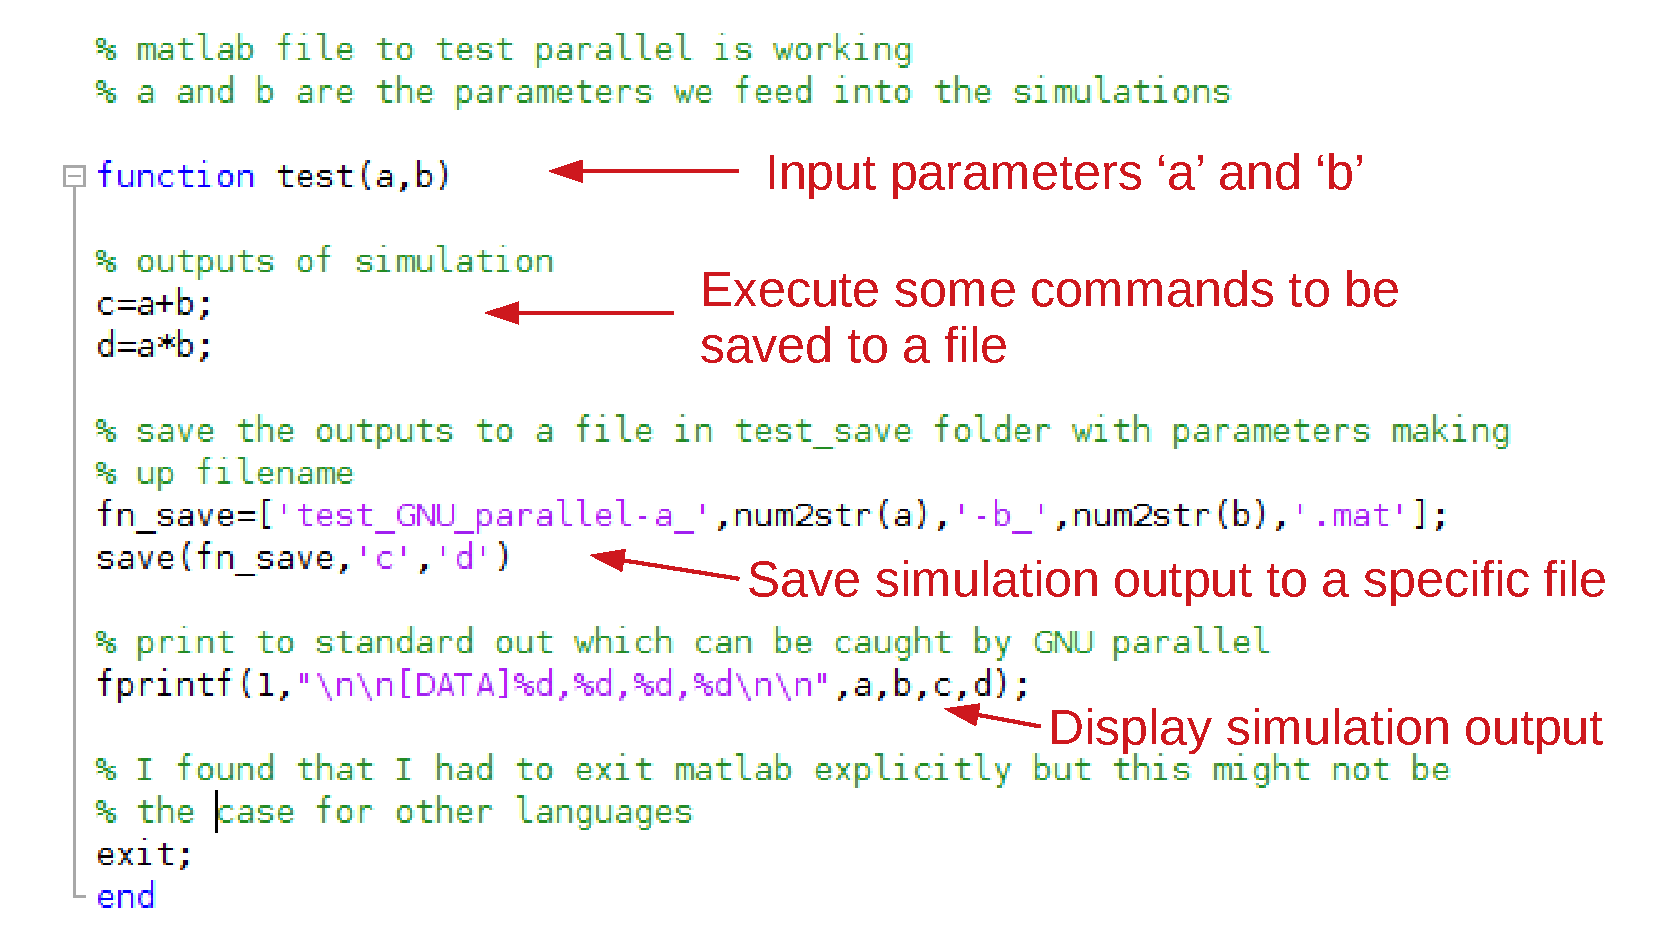
\includegraphics[width=.8\linewidth]{figures/matlab_code_annotated.pdf}	
\end{figure}

\end{frame}

\begin{frame}{Example: Creating a shell script to run a single instance of the Matlab script}
\begin{itemize}
	\item Create a new shell script (\texttt{run\_test\_matlab.sh}) to initiate the Matlab simulation:
\begin{figure}
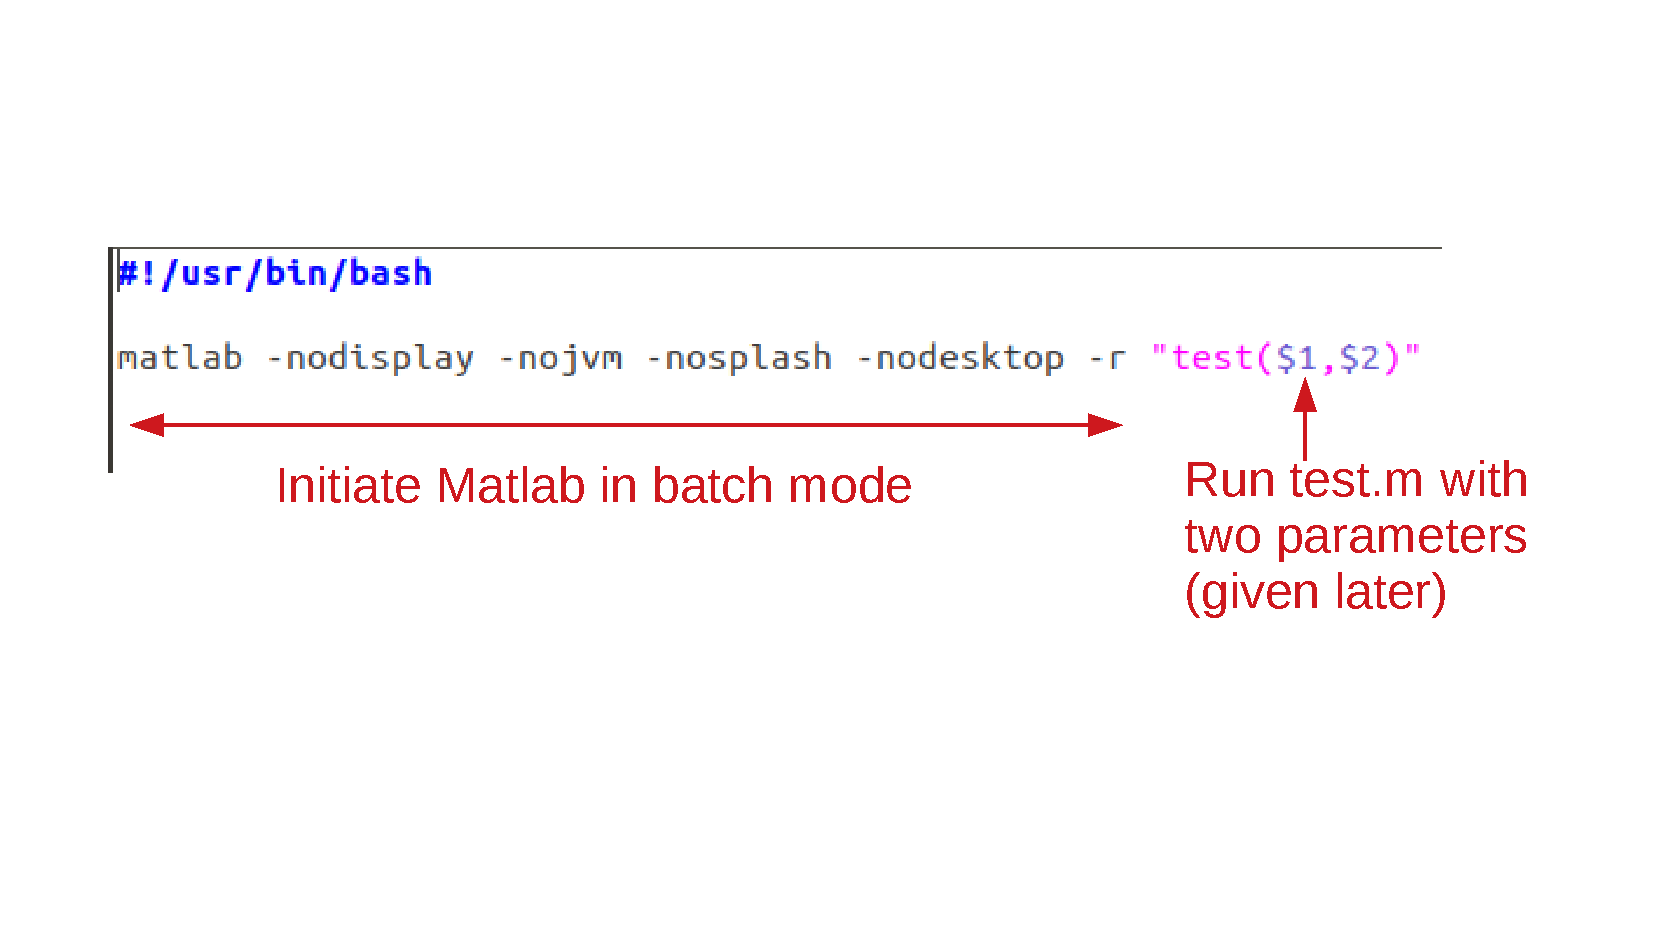
\includegraphics[clip,trim=0in 2in 0in 2in,width=0.8\linewidth]{figures/run_matlab_sh_annotated.pdf}
\end{figure}
\item Make sure this file is executable. If not, on the command line execute \\ \texttt{chmod u=rwx run\_test\_matlab.sh}
\end{itemize}
\end{frame}

\begin{frame}{Example: Creating a parameter file with all necessary parameters}
\begin{itemize}
	\item Create a file called \texttt{parameters.txt} containing all the parameters for the simulation
	\item I am using a comma separated format (I tell GNU parallel this later)
\end{itemize}
\begin{figure}
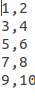
\includegraphics[width=.05\linewidth]{figures/parameter_file.png}
\end{figure}
\end{frame}

\begin{frame}{Example: Creating a shell script to run multiple simulations in parallel}
\begin{itemize}
	\item Create a new shell script (\texttt{test\_parallel\_1host.sh}) to run the Matlab simulation simultaneously:
	\begin{figure}
		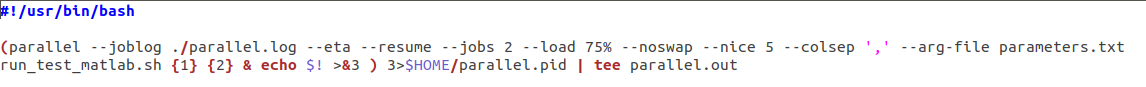
\includegraphics[width=\linewidth]{figures/run_parallel.png}
	\end{figure}
\item Make sure this file is executable. If not, on the command line execute \\ \texttt{chmod u=rwx test\_parallel\_1host.sh}
\item \texttt{--jobs 2 --load 50\% --noswap --nice 5} means
run a maximum of two jobs concurrently on each server, each with a nice value of 5 (sets priority of jobs) and only start a new job if the load on the machine is less than 75\% (considers the number of CPUs)
don't start jobs if the system is swapping
\end{itemize}
\end{frame}

\begin{frame}{Example: Add folder with shell scripts to \texttt{\$PATH}}
\begin{itemize}
	\item This allows us to run the shell script from any folder 
\end{itemize}
\end{frame}

\begin{frame}{Example: Run GNU parallel}
\begin{itemize}
	\item Make sure \texttt{test.m} and \texttt{parameters.txt} are in the current working directory
	\item Execute \texttt{test\_parallel\_1host.sh} on the command line to run $5$ Matlab simulations, $2$ at a time.
	\item As one simulation finishes GNU parallel automatically spawns the next simulation in the queue
	\item Execute \texttt{clean\_stdout.sh} to extract the data displayed in standard out and save it in a comma separated list
\end{itemize}
\end{frame}

%\begin{frame}{Background on concurrency and parallelism}
%\url{https://vimeo.com/49718712}
%\end{frame}


\end{document}

%\begin{figure}
%	\subfigure[]{\includegraphics[clip,trim=2.5in 0in 2.5in 0in, width=0.3\linewidth]{bio_model_orai_influx_no_PMCA.pdf}
%		\label{fig:intro:ill:Orai_influx}			
%	}	
%	\subfigure[]{\includegraphics[clip,trim=2.5in 0in 2.5in 0in, width=0.3\linewidth]{bio_model_activated_pumps_no_PMCA.pdf}
%		\label{fig:intro:ill:Orai_influx_SERCA_uptake}
%	}		
%	\subfigure[]{\includegraphics[clip,trim=2.5in 0in 2.5in 0in, width=0.3\linewidth]{bio_model_refill_no_PMCA.pdf}
%		\label{fig:intro:ill:Refilling}
%	}	
%	\caption{(a) Orai channels on PM open. (b) Increased \ca in ER-PM junction activates SERCA pumps on ER membrane. (c) Activated SERCA pumps refill ER}		
%\end{figure}